\documentclass[a4paper,12pt]{article}

\usepackage[slovene]{babel}
\usepackage{amsfonts,amssymb,amsmath}
\usepackage{amsthm}
\usepackage[utf8]{inputenc}
\usepackage[T1]{fontenc}
\usepackage{lmodern}
\usepackage{graphicx}
\graphicspath{{./images/}}

\usepackage{tikz-cd}

\usetikzlibrary{babel}

\def\N{\mathbb{N}} % mnozica naravnih stevil
\def\Z{\mathbb{Z}} % mnozica celih stevil
\def\Q{\mathbb{Q}} % mnozica racionalnih stevil
\def\R{\mathbb{R}} % mnozica realnih stevil
\def\C{\mathbb{C}} % mnozica kompleksnih stevil


\newcommand{\cay}[2]{$Cay(#1, #2)$}
\newcommand{\aut}[2]{Aut(#1, #2)}
\newcommand{\cit}[1]{(Izrek \ref{#1})}
\newcommand{\St}{\widetilde{S}}
\newcommand{\As}{A^*}
\newcommand{\Freds}{F_{red}(S)}
\newcommand{\geslo}[2]{\noindent\textbf{#1} \quad \hangindent=1cm #2\\[-1pc]}


\def\qed{$\hfill\Box$}   % konec dokaza
\def\qedm{\qquad\Box}   % konec dokaza v matematičnem načinu
\newtheorem{izrek}{Izrek}
\newtheorem{trditev}{Trditev}
\newtheorem{posledica}{Posledica}
\newtheorem{lema}{Lema}
\newtheorem{opomba}{Opomba}
\newtheorem{definicija}{Definicija}
\newtheorem{zgled}{Zgled}

\title{Proste grupe in drevesa \\ 
\Large Seminar}
\author{Jakob Pogačnik Souvent \\
Fakulteta za matematiko in fiziko \\
Oddelek za matematiko}





\begin{document}


%%%%%%%%%%%%%%%%%%%%%%%%%%%%%%%%%%%%%%%%%%%%%%%%%%%%%%%%%%%%%%%%%%%%%


\maketitle


%%%%%%%%%%%%%%%%%%%%%%%%%%%%%%%%%%%%%%%%%%%%%%%%%%%%%%%%%%%%%%%%%%%%%

\section{Uvod}

V študiju algebraičnih struktur imajo poseben pomen strukture, ki jih lahko opišemno z neko množico generatorjev,
ki so med seboj čim manj povezani. To so t.i. \textbf{proste} strukture.

V vektorskoh prostorih, denimo, nepovezanost elementov pojmujemo kot njihovo linearno neodvisnost.
In ker ima vsak končnorazsežni vektorski prostor bazo iz linearno neodvisnih vektorjev, ima kot tak, obliko proste strukture.

V članku se bomo ukvarjali predvsem s problemom prepoznavanja prostih struktur znotraj teorije grup.
Izkaže se namreč, da za razliko od vektorskih prostorov, nima vsaka grupa oblike proste strukture, kar je eden izmed razlogov, zakaj je teorija grup nekoliko bolj zapletena kot študij vektorskih prostorov.


\section{Proste grupe}

Preden se lahko lotimo problema iskanja prostih struktur v teoriji grup, rabimo najprej postaviti definicijo \textbf{proste grupe}.

\begin{definicija}[Prosta grupa]
    Naj bo $S$ množica. Za grupo $F$, ki vsebuje $S$ Pravimo, da $S$ \textbf{prosto generira} $F$, če velja:

    Za vsako grupo $G$ in vsako preslikavo $\varphi : S \longrightarrow G$ obstaja enolično določen homomorfizem $\overline{\varphi} : F \longrightarrow G$, ki razširi $\varphi$. %(torej $\overline{\varphi}|_{S} = \varphi$)

    $$
    \begin{tikzcd}
        S && G \\
        &&& {} \\
        F
        \arrow["{\overline{\varphi}}"', dashed, from=3-1, to=1-3]
        \arrow["\varphi"', from=1-1, to=1-3]
        \arrow[hook, from=1-1, to=3-1]
    \end{tikzcd}
    $$

    Grupi $F$ pravimo \textbf{prosta}, če vsebuje kakšno podmnožico, ki jo prosto generira, zgornji lastnosti pa pravimo \textbf{univerzalna lastnost prostih grup}.
\end{definicija}

Če imamo pri branju zgornje definicije v mislih analogijo z vektorskimi prostori, lahko na elemente množice $S$ gledamo kot na bazne vektore.
Univerzalna lastnost nam potem pove, da je homomorfizem proste grupe enolično definiran s slikami ``baznih vektorjev``.

\begin{opomba}
    V definiciji ne zahtevamo, da je množica $S$ množica generatorjev grupe $F$, vendar bomo videli, da to sledi iz zahtevane univerzalne lastnosti (glej Izrek \ref{izr:generator}).
\end{opomba}

Da utrdimo pojem proste grupe, si oglejmo nekaj zgledov.

\begin{zgled}
\label{zgl:grupe}
    \hfill
        \begin{enumerate}
            \item Trivialna grupa je prosto generirana s prazno množico.
            \item $\Z$ je prosta grupa.
            % o generirana z $\{1\}$, vendar ne z $\{2, 3\}$ ali z $\{2\}$

            Pri dokazu da $\Z$ je prosta grupa je dovolj, da najdemo neko množico ki jo prosto generira.
            Denimo $S := \{1\}$. Vzemimo poljubno preslikavo $\varphi : S \longrightarrow G$, kjer je $G$ poljubna grupa.
            Če $\varphi(1) = e$ je trivialni homomorfizem $\overline{\varphi}(n) = e$ ustrezna razširitev.
            Če pa $\varphi(1) = g_0 \neq e$ predpis $\overline{\varphi}(n) = g_0^n$ ustrezno razširi $\varphi$.

            Omembe vredno je, da univerzalne lastnosti ne izpolnjuje vsaka podmnožica proste grupe. Niti je ne izpolnjuje vsaka podmnožica generatorjev.
            Če bi naprimer vzeli $S := \{2, 3\}$ za preslikavo $\varphi : S \longrightarrow \Z_2$ definirano kot $\varphi(2) = 1$ in $\varphi(3) = 1$
            ne obstaja homomorfizem ki na $S$ sovpada s $\varphi$. Če bi namreč obstajala razširitev $\overline{\varphi}$, bi moralo veljati
            $$\overline{\varphi}(1) = \overline{\varphi}(3 - 2) = \overline{\varphi}(3) - \overline{\varphi}(2) = 1 - 1 = 0\text{,}$$
            kar pa vodi v protislovje, ker
            $$\overline{\varphi}(2) = \overline{\varphi}(1 + 1) = \overline{\varphi}(1) + \overline{\varphi}(1) = 1 + 1 = 0 \neq 1 = \varphi(2)\text{.}$$

            \item $\Z_2$ ni prosto generirana.
            
            Za $\Z_2$ imamo samo $3$ možne kandidate za množico $S$. To so $S_1 = \{0\}$, $S_2 = \{0, 1\}$ in $S_3 = \{1\}$.
            Hitro se prepričamo, da $S_1$ in $S_2$ nista ustrezna, saj lahko v tem primeru za preslikavo $\varphi$ izberemo tako preslikavo v netrivialno grupo $G$, ki $0$ ne slika v enoto.
            Ker homomorfizem slika enoto $\varphi$ torej ne moremo razširiti do homomorfizma.
            Opazimo, da množica $S$, ki prosto generira grupo $F$, ne more vsebovati enote.

            Poiščimo še protiprimer za $S_3$. Definirajmo preslikavo $\varphi : S_3 \longrightarrow \Z$ s predpisom $\varphi(1) = 2$. Če obstaja $\overline{\varphi}$ ki na $S$ sovpada s $\varphi$ mora veljati
            $$
            \overline{\varphi}(0) = \overline{\varphi}(1 + 1) = \overline{\varphi}(1) + \overline{\varphi}(1) = 2 + 2 = 4
            $$
            kar pa je protislovje, saj mora homomorfizem slikati enoto v enoto.
        \end{enumerate}
\end{zgled}

Oglejmo nekaj osnovnih lastnosti prostih grup, ki jih bomo potrebovali v kasnejših dokazih.

\begin{izrek}[Enoličnost prostih grup]
    \label{izr:enolicnost}
    Naj bo $S$ množica. Potem do izomorfizma natančno obstaja največ ena grupa prosto generirana z $S$.
\end{izrek}

\begin{proof}
    Naj bosta $F$ in $F'$ grupi, prosto generirani z množico $S$. Naj bosta $\varphi : S \hookrightarrow F$ in $\varphi' : S \hookrightarrow F'$ inkluziji.
    Po univerzalni lasnosti prostih grup lahko $\varphi$ in $\varphi'$ razširimo do homomorfizmov $\overline{\varphi}$ in $\overline{\varphi'}$.

    $$
    \begin{tikzcd}
        S && {F'} \\
        &&& {} \\
        F
        \arrow["{\varphi'}", from=1-1, to=1-3]
        \arrow["\varphi"', hook, from=1-1, to=3-1]
        \arrow["{\overline{\varphi}'}"', dashed, from=3-1, to=1-3]
    \end{tikzcd}
    \hspace{40pt}
    \begin{tikzcd}
        S && F \\
        &&& {} \\
        {F'}
        \arrow["{\overline{\varphi}}"', dashed, from=3-1, to=1-3]
        \arrow["\varphi"', from=1-1, to=1-3]
        \arrow["{\varphi'}", hook, from=1-1, to=3-1]
    \end{tikzcd}
    $$

    Kompozitum homomorfizmov $\overline{\varphi} \circ \overline{\varphi}' : F \rightarrow F$ je homomorfizem, ki je na $S$ identiteta ($\overline{\varphi}$ in $\overline{\varphi}'$ na $S$ sovpadata z $\varphi$ in $\varphi'$).
    Če na $\varphi$ gledamo kot na preslikavo iz $S$ v $F$ sta torej tako $\overline{\varphi} \circ \overline{\varphi}'$ kot $id_F$ razširitvi, ki ustrezata univerzalni lastnosti in zato po enoličnosti razširitve velja $\overline{\varphi} \circ \overline{\varphi}' = id_F$.
    
    $$
    \begin{tikzcd}
        S && F \\
        &&& {} \\
        F
        \arrow["{\overline{\varphi} \circ \overline{\varphi}'}"', dashed, from=3-1, to=1-3]
        \arrow["\varphi"', from=1-1, to=1-3]
        \arrow["\varphi", hook, from=1-1, to=3-1]
    \end{tikzcd}
    \hspace{40pt}
    \begin{tikzcd}
        S && F \\
        &&& {} \\
        F
        \arrow["id_F"', dashed, from=3-1, to=1-3]
        \arrow["\varphi"', from=1-1, to=1-3]
        \arrow["\varphi", hook, from=1-1, to=3-1]
    \end{tikzcd}
    $$

    Podobno $\overline{\varphi}' \circ \overline{\varphi} = id_{F'}$, torej je $\overline{\varphi} \circ \overline{\varphi}'$ izomorfizem.
\end{proof}

\begin{izrek}[Eksistenca prostih grup]
\label{izr:freeGroupExistence}
    Naj bo $S$ množica. Potem obstaja grupa, prosto generirana z $S$.
\end{izrek}

\begin{opomba}
    Po izreku \ref{izr:enolicnost} je ta grupa enolično določena do izomorfizma natančno.
\end{opomba}

\begin{proof}
    Ideja dokaza je konstrukcija grupe sestavljene iz t.i. \textit{besed}, ki so sestavljene iz elementov množice $S$ in njihovih inverzov, na katerih bomo uporabili le neposredno pravilo krajšanja.

    Konkretno definiramo
    $$
    A := S \cup \widehat{S}
    $$
    kot abecedo iz katere bomo sestavili naše besede. Tu $\widehat{S} = \{\widehat{s} \; | \; s \in S\}$ predstavlja disjunktno kopijo $S$ (t.j. $\widehat{\cdot} : S \longrightarrow \widehat{S}$ je bijekcija in $S \bigcap \widehat{S} = \emptyset$), ki bo v konstrukciji prevzela vlogo inverzov.

    V prvem koraku vzemimo z oznako $\As$ množico vseh končnih zaporedij iz abecede $A$. To vsebuje, med drugimi, tudi prazno besedo $\varepsilon$.
    Na $\As$ definirajmo binarno operacijo kompozicije, ki stakne skupaj dve besedi. Ta operacija je asociativna in $\varepsilon$ je nevtralni element.

    V nadaljevanju definirajmo
    $$
    F(S) := \As / \sim
    $$
    kjer je $\sim$ ekvivalenčna relacija, definirana kot
    \begin{align*}
        \forall x, y \in \As \; \forall s \in S : xs\widehat{s}y \sim xy \\
        \forall x, y \in \As \; \forall s \in S : x\widehat{s}sy \sim xy\text{.}
    \end{align*}
    Drugače, elementa v $\As$ obravnavamo kot ekvivalentna, če se razlikujeta natanko za neposredno uporabo pravila krajšanja (Opomba: popolnoma formalno za $\sim$ vzamemo najmanjšo ekvivalenčno relacijo, ki zadostuje zgornjemu pogoju).
    
    Ni težko preveriti, da kompozicija besed v $\As$ inducira dobro definirano binarno operacijo $\cdot : F(S) \times F(S) \longrightarrow F(S)$ definirano kot
    $$
    [x] \cdot [y] = [xy]
    $$
    kjer so z oglatimi oklepaji označeni ekvivalenčni razredi po $\sim$.

    Pokažimo, da je množica $F(S)$ s tako operacijo grupa. Očitno je $[\varepsilon]$ nevtralni element, asociativnost pa sledi iz asociativnosti kompozicije v $\As$.
    Induktivno (po dolžini besede) definiramo preslikavo $I : \As \longrightarrow \As$, ki besedi priredi inverz kot
    \begin{align*}
        I(\varepsilon) &= \varepsilon \\
        I(sx) &:= I(x)\widehat{s} \\
        I(\widehat{s}x) &:= I(x)s
    \end{align*}
    za vse $x \in \As$ in $s \in S$. Induktivno vidimo da $I(I(x)) = x$ in
    $$
    [I(x)] \cdot [x] = [I(x)x] = [\varepsilon]
    $$
    za vse $x \in \As$ (zadnja enakost sledi iz definicije $\sim$). Zato tudi
    $$
    [x] \cdot [I(x)] = [I(I(x))] \cdot [I(x)] = [\varepsilon] \text{.}
    $$
    Torej je $F(S)$ grupa.

    Ostane name le še pokazati, da $S$ prosto generira $F(S)$.
    Naj bo $i : S \longrightarrow F(S)$ preslikava, ki vsaki črki $S \subset \As$ priredi njen ekvivalenčni razred v $F(S)$.
    Po konstrukciji je $i(S)$ množica generatorjev $F(S)$.
    
    Zdaj pokažimo, da ima $F(S)$ naslednjo lastnost, podobno univerzalni lastnosti prostih grup: za vsako grupo $G$ in preslikavo $\varphi : S \longrightarrow G$
    obstaja enolično določen homomorfizem grup $\overline{\varphi} : F(S) \longrightarrow G$, da $\varphi = \overline{\varphi} \circ i$.
    $$
    \begin{tikzcd}
        S && G \\
        &&& {} \\
        {F(S)}
        \arrow["{\overline{\varphi}}"', dashed, from=3-1, to=1-3]
        \arrow["\varphi"', from=1-1, to=1-3]
        \arrow["i", from=1-1, to=3-1]
    \end{tikzcd}
    $$
    Opomnimo, da formalno gledano to ni univerzalna lastnost prostih grup, saj grupa $F(S)$ ne vsebuje množice $S$, temveč njej ustrezne ekvivalenčne razrede $i(S)$. Če je $i$ injektivna, pa lahko $S$ identificiramo z $i(S)$ in to res postane univerzalna lastnost.

    Pri dokazu zgornje lastnosti z danim $\varphi$ induktivno definiramo
    \begin{align*}
        \varphi^* : \As &\longrightarrow G \\
        \varepsilon &\longmapsto e \\
        sx &\longmapsto \varphi(s) \cdot \varphi^*(x) \\
        \widehat{s}x &\longmapsto (\varphi(s))^{-1} \cdot \varphi^*(x)
    \end{align*}
    za vse $s \in S$ in vse $x \in \As$. Lahko je videti, da je $\varphi^*$ kompatibilna z ekvivalenčno relacijo $\sim$ in da $\varphi^*(xy) = \varphi^*(x) \cdot \varphi^*(y)$.
    Torej $\varphi^*$ inducira dobro definiran homomorfizem
    \begin{align*}
    \overline{\varphi} : F(S) &\longrightarrow G \\
    [x] &\longmapsto [\varphi^*(x)] \text{.}
    \end{align*}
    Po konstrukciji je $\varphi = \overline{\varphi} \circ i$. Ker $i(S)$ generira $F(S)$, pa je $\overline{\varphi}$ enolično določen.

    Ostane nam le še dokaz injektivnosti $i$.
    Naj bosta $s_1, s_2 \in S$ in $\varphi : S \longrightarrow \Z$ poljubna preslikava, da velja $\varphi(s_1) = 1$ in $\varphi(s_2) = -1$.
    Potem nam inducirani $\overline{\varphi}$ da
    $$
    \overline{\varphi}(i(s_1)) = \varphi(s_1) = 1 \neq -1 = \varphi(s_2) = \overline{\varphi}(i(s_2)) \text{.}
    $$
    Oziroma $i(s_1) \neq i(s_2)$.
    
    Torej je $i$ injektivna in lahko $S$ identificiramo z njegovo sliko $i(S)$, zgornja lastnost pa tako res postane univerzalna lastnost prostih grup.
\end{proof}

\begin{izrek}
\label{izr:generator}
    Naj bo $F$ grupa, prosto generirana z $S$. Potem je $S$ množica generatorjev grupe $F$.
\end{izrek}

\begin{proof}
    Po konstrukciji trditev velja za prosto grupo $F(S)$, ki je generirana z $S$ (glej dokaz izreka \ref{izr:freeGroupExistence}). Po izreku o enoličnosti prostih gruop (glej izrek \ref{izr:enolicnost}), obstaja izomorfizem med $F(S) \cong F$, ki je na $S$ identiteta,
    iz česar sledi, da je $S$ množica generatorjev grupe $F$.
\end{proof}

% Preden začnemo delati s prostimi grupami si poglejmo še alternativno konstrukcijo, ki nam bo pomagala pri razumevanju izrekov.

Ker je formalno delo s kvocientno grupo, ki smo jo dobili pri konstrukciji v izreku \ref{izr:freeGroupExistence},
nekoliko zamudno in težje razumljivo, brez dokaza privzemimo naslednjo trditev,
ki nam bo nudila ekvivalentno reprezentacijo grupe, prosto generirane s poljubno množico $S$.

Če bralca zanima dokaz, naj se obrne na dokaz trditve 3.3.5 v članku \cite{Loh}.

\begin{definicija}[Okrajšana beseda]
    Naj bo $S$ množica in $(S \cup \widehat{S})^*$ množica vseh besed nad elementi $S$ in njihovimi formalnimi inverzi.
    Naj bo $n \in \N$ in $s_1, \ldots, s_n \in S \cup \widehat{S}$. Za besedo $s_1 \ldots s_n$ pravimo, da je \textbf{okrajšana}, če velja
    $$
    s_{j+1} \neq \widehat{s}_j \quad \text{in} \quad \widehat{s}_{j+1} \neq s_j
    $$
    za vse $j \in \{1, \ldots, n-1\}$. Posebej: $\varepsilon$ je okrajšana.

    Množico vseh okrajšanih besed v $(S \cup \widehat{S})^*$ označimo z $\Freds$.
\end{definicija}

\begin{trditev}
    Naj bo $S$ množica.
    \begin{enumerate}
        \item Množica okrajšanih besed $\Freds$ nad $S \cup \widehat{S}$ tvori grupo za operacijo kompozicije, definirano kot
        \begin{align*}
            \Freds \times \Freds &\longrightarrow \Freds \\
            (s_1 \ldots s_n, s_{n+1} \ldots s_m) &\longmapsto (s_1 \ldots s_{n-r} s_{n+1+r} \ldots s_{m})
        \end{align*}
        kjer so $s_1, \ldots, s_m \in S \cup \widehat{S}$ in je $r$ največje tako število, da za vsak $j \in \{0, \ldots, r-1\}$ velja
        $$
        s_{n-j} = \widehat{s}_{n+1+j} \quad \text{ali} \quad \widehat{s}_{n-j} = s_{n+1+j} \text{.}
        $$
        Z drugimi besedami, kompozicija je definirana s konkatinacijo dveh besed in nato okrajšavo največjega možnega števila elementov na mestu konkatinacije.
        
        \item Grupa $\Freds$ je prosto generirana z $S$.
    \end{enumerate}
\end{trditev}

Množico $\Freds$ torej dobimo tako, da se v $F(S)$ omejimo na enega predstavnika vsakega ekvivalenčnega razreda.
To nam nekoliko okrajša delo v nadaljnjih izrekih, saj smo delo z ekvivalenčnimi razredi prevedli na delo s predstavnikom,
kar nam v dokazih prihrani dokaz dobre definiranosti lastnosti oz. operacij na ekvivalenčnih razredih.

% \begin{posledica}
%     Naj bo $S$ množica. Vsak element proste grupe $F(S) = (S \cup \widehat{S})^* / \sim$ ustreza natanko eni okrajšani besedi nad $S \cup \widehat{S}$.
% \end{posledica}
%
% \begin{proof}
%     Iz izreka \ref{izr:enolicnost} sledi $F(S) \cong \Freds$.
% \end{proof}

\section{Cayleyjevi grafi}

Eno izmed temeljnih vprašanj v teoriji grup je, kako si grupe predstavljati kot geometrijske objekte.
Eden izmed načinov, kako to storimo, je z uporabo cayleyevih grafov, ki opišejo relacije med elementi grupe
glede na njeno množico generatorjev.

Preden definiramo cayleyeve grafe, zapišimo še definiciji za pot in cikel v grafu.
V cayleyevih grafih bodo vlogo vozlišč zavzeli elementi grupe, vlogo povezav pa relacije med njimi, zato je koristno, da privzamemo tako definicijo
poti in ciklov, ki nam bo izolirala elemente grupe.

\begin{definicija}[Pot]
    \textbf{Pot} ki povezuje vozlišči $v_{0}$ in $v_{n}$ v grafu $X = (V, E)$, je zaporedje paroma različnih vozlišč $v_{0},\dots,v_{n} \in V$, za
    katerega velja, da je $\{v_{i}, v_{i+1}\} \in E$ za vsak $i \in \{0, \dots, n-1 \}$.
\end{definicija}

\begin{definicija}[Cikel]
    Naj bo $n \in \N$, $n > 2$. \textbf{Cikel} v grafu $X = (V, E)$ dolžine $n$ je pot $v_{0},\dots,v_{n}$ v $X$, za katero velja $\{v_{n-1}, v_n\} \in E$.
\end{definicija}

\begin{definicija}[Cayleyev graf]
    Naj bo $S$ podmnožica, ki generira grupo $G$. \textbf{Cayleyjev graf} $G$ glede na množico generatorjev $S$ je graf \cay{G}{S}, katerega množica vozlišč je množica $G$
    in katerega množica povezav je množica
    $$
    \{\{g, g \cdot s\}\;|\;g \in G, s \in (S \cup S^{-1}) \setminus \{e\} \},
    $$
    kjer je s $\cdot$ označeno množenje v grupi $G$.
\end{definicija}

Dve vozlišči v Cayleyjevem grafu sta si torej sosednji natanko tedaj, ko se razlikujeta le za desno množenje z elementom (ali inverzom) dane množice $S$.

Za boljšo predstavo si oglejmo cayleyeve grafe nekaterih nam že znanih grup.

\begin{zgled}
    Cayleyevi grafi nekaterih dobro znanih grup.
    \begin{enumerate}
        \item \cay{\Z}{\{1\}}
        
        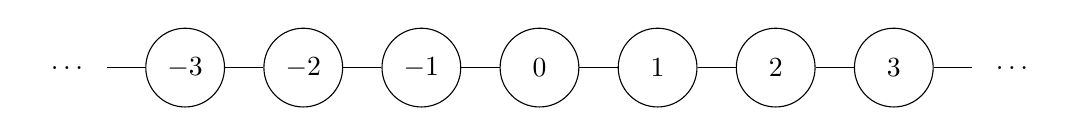
\begin{tikzpicture}[node distance={15mm}, main/.style = {draw, circle}] 
            \node[main,minimum size=1cm] (1) {$-3$};
            \node[main,minimum size=1cm] (2) [right of=1] {$-2$};
            \node[main,minimum size=1cm] (3) [right of=2] {$-1$}; 
            \node[main,minimum size=1cm] (4) [right of=3] {$0$};
            \node[main,minimum size=1cm] (5) [right of=4] {$1$}; 
            \node[main,minimum size=1cm] (6) [right of=5] {$2$};
            \node[main,minimum size=1cm] (7) [right of=6] {$3$};

            \node[main,minimum size=1cm, draw=none] (8) [right of=7] {$\ldots$};
            \node[main,minimum size=1cm, draw=none] (9) [left of=1] {$\ldots$};

            \draw (1) -- (2);
            \draw (2) -- (3);
            \draw (3) -- (4);
            \draw (4) -- (5);
            \draw (5) -- (6);
            \draw (6) -- (7);
            
            \draw (1) -- (9);
            \draw (7) -- (8);
            
        \end{tikzpicture} 
            

        \item \cay{\Z}{\{2,3\}}
        
        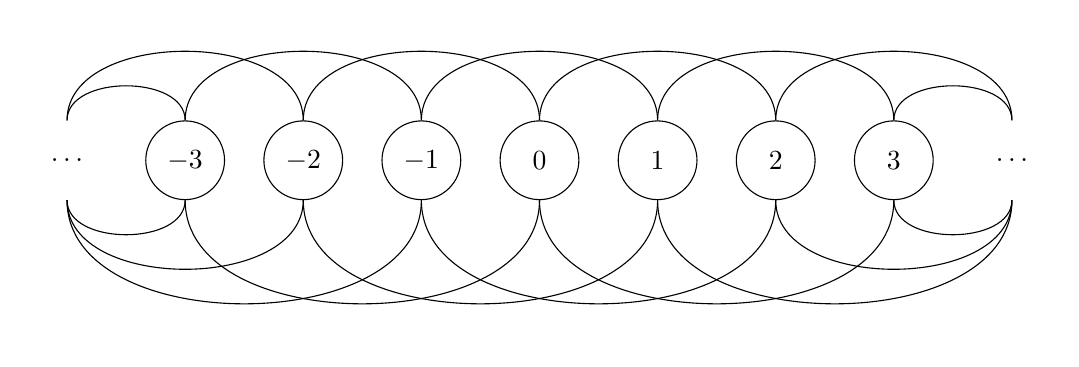
\begin{tikzpicture}[node distance={15mm}, main/.style = {draw, circle}] 
            \node[main,minimum size=1cm] (1) {$-3$};
            \node[main,minimum size=1cm] (2) [right of=1] {$-2$};
            \node[main,minimum size=1cm] (3) [right of=2] {$-1$}; 
            \node[main,minimum size=1cm] (4) [right of=3] {$0$};
            \node[main,minimum size=1cm] (5) [right of=4] {$1$}; 
            \node[main,minimum size=1cm] (6) [right of=5] {$2$};
            \node[main,minimum size=1cm] (7) [right of=6] {$3$};
            
            \node[main,minimum size=1cm, draw=none] (8) [right of=7] {$\ldots$};
            \node[main,minimum size=1cm, draw=none] (9) [left of=1] {$\ldots$};

            \draw (1) to [out=90,in=90,looseness=1] (3);
            \draw (1) to [out=270,in=270,looseness=1] (4);

            \draw (2) to [out=90,in=90,looseness=1] (4);
            \draw (2) to [out=270,in=270,looseness=1] (5);

            \draw (3) to [out=90,in=90,looseness=1] (5);
            \draw (3) to [out=270,in=270,looseness=1] (6);

            \draw (4) to [out=90,in=90,looseness=1] (6);
            \draw (4) to [out=270,in=270,looseness=1] (7);
            
            \draw (5) to [out=90,in=90,looseness=1] (7);
            
            \draw (9) to [out=90,in=90,looseness=1] (1);
            \draw (9) to [out=90,in=90,looseness=1] (2);

            \draw (9) to [out=270,in=270,looseness=1] (1);
            \draw (9) to [out=270,in=270,looseness=1] (2);
            \draw (9) to [out=270,in=270,looseness=1] (3);
            
            \draw (8) to [out=90,in=90,looseness=1] (7);
            \draw (8) to [out=90,in=90,looseness=1] (6);

            \draw (8) to [out=270,in=270,looseness=1] (7);
            \draw (8) to [out=270,in=270,looseness=1] (6);
            \draw (8) to [out=270,in=270,looseness=1] (5);


            
        \end{tikzpicture} 

        Vidimo, da cayleyev graf ni odvisen le od grupe, temveč tudi od množice generatorjev ki jo vzamemo.

        \item \cay{\Z_6}{\{1\}}
        
        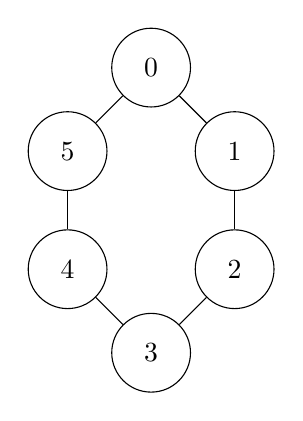
\begin{tikzpicture}[node distance={15mm}, main/.style = {draw, circle}] 
            \node[main,minimum size=1cm] (1) {$0$};
            \node[main,minimum size=1cm] (2) [below right of=1] {$1$};
            \node[main,minimum size=1cm] (3) [below of=2] {$2$}; 
            \node[main,minimum size=1cm] (4) [below left of=3] {$3$};
            \node[main,minimum size=1cm] (5) [below left of=1] {$5$}; 
            \node[main,minimum size=1cm] (6) [below of=5] {$4$};
            
            \draw (1) to (2);
            \draw (2) to (3);
            \draw (3) to (4);
            \draw (1) to (5);
            \draw (5) to (6);
            \draw (5) to (6);
            \draw (4) to (6);

            
        \end{tikzpicture} 


    \end{enumerate}
\end{zgled}

Seveda pa nas v tem članku ne zanimajo katerekoli grupe, temveč proste grupe.
Naravno se torej porodi vprašanje, kako izgleda cayleyev graf proste grupe glede na množico, ki jo prosto generira
(po izreku \ref{izr:generator} ta množica generira grupo)?
Povezave v cayleyevim grafu namreč predstavljajo relacije med elementi grupe, glede na množico generatorjev,
v prostih grupah pa generatorji med seboj nimajo relacij.

Če torej poskusimo skicirati graf neke proste grupe dobimo skico podobno sliki \ref{fig:cayleyGraph}.
Opazimo, da se odsotnost relacij med generatorji v grafu izraža kot odsotnost povezav med elementi,
kar porodi najmanjši možen povezan graf, drevo.

Našo ugotovitev zapišemo v izrek in jo tudi formalno dokažemo.

\begin{figure}[!htp]
    \centering
    \includegraphics[width=0.6\textwidth]{FreeGroupCayley.png}
    \caption{Cayleyev graf proste grupe \cay{\Freds}{\{a,b\}}}
    \label{fig:cayleyGraph}
\end{figure}
    

\begin{izrek}
    \label{izr:freeCayleyTree}
    Naj bo $F$ grupa, prosto generirana z $S \subset F$. Potem je graf \cay{F}{S} drevo.
\end{izrek}

\begin{proof}
    Brez škode za splošnost se omejimo na $\Freds$, saj sta $F \cong \Freds$ izomorfna.
    Če imamo v grafu \cay{\Freds}{S} cikel, to pomeni, da lahko začnemo v nekem vozlišču $x$ in z zaporednim množenjem 
    z elementi $S$ (elementa sta sosednja natanko tedaj ko se razlikujeta za množenje z nekim elementom $S$) pridemo nazaj v $x$. Torej
    $$
        x s_1 \ldots s_n = x\text{.}
    $$
    Okrajšamo $x$ in dobimo
    $$
    s_1 \ldots s_n = \varepsilon \text{,}
    $$
    % TODO lahko imamo a b i(b) i(a) inverzi niso nujno zaporedni
    kar pa je protislovno, saj je v $\Freds$ to možno natanko tedaj, ko so si ustrezni sosedni elementi inverzni (inverz pa pomeni potovanje po isti povezavi v obratno smer s čimer pridemo v protislovje z enoličnostjo vozlišč v ciklu).
\end{proof}

\begin{opomba}
    Obrat v splošnem ne drži, t.j. ni res da za vsak \cay{F}{S} sledi, da je $F$ prosto generirana z $S$.
    Protiprimer bi bil denimo \cay{\Z_2}{\{1\}}.
\end{opomba}

Kljub temu pa lahko pridemo do obrata, če poleg drevesne strukture dodamo predpostavko,
da se nobena elementa množice $S$ ne zmnožita v enoto. Tako se izognemo primerom,
ko bi ustvarili cikel dolžine $2$, kar nam v posebnih primerih (kot \cay{\Z_2}{\{1\}} zgoraj), ker v povezavah ne ločimo usmerjenosti, ustvari graf, ki ustreza definiciji drevesa.

\begin{izrek}[Obrat]
\label{izr:cayleyFreeCycle}
    Naj bo $G$ grupa in naj bo $S \subset G$ množica generatorjev $G$.
    Dodatno naj velja, da $s \cdot t \neq e$ za vsaka $s, t \in S$.

    Če je Cayleyev graf \cay{G}{S} drevo, potem $S$ prosto generira $G$.
\end{izrek}

\begin{proof}
    Naj bo $G$ grupa in $S \subset G$ taka da, velja predpostavka izreka.
    Da pokažemo, da je $G$ prosto generirana, je dovolj, da pokažemo, da je $G$ izomorfna $\Freds$ z izomorfizmom, ki je na $S$ identiteta.

    Ker je $\Freds$ prosto generirana z $S$ nam univerzalna lastnost prostih grup že nudi obetavnega kandidata za izomorfizem, t.j. homomorfizem $\overline{\varphi}$, ki ga
    dobimo z razširitvijo identitete $\varphi : S \longrightarrow G$. Ker je po predpostavki $S$ množica generatorjev $G$, hitro sledi, da je $\overline{\varphi}$ surjektiven.

    Predpostavimo da $\overline{\varphi}$ ni injektiven. Potem obstajata neka $s_1 \ldots s_n \in \Freds \setminus \{\varepsilon\}$, kjer $s_1, \ldots, s_n \in S \cup \widehat{S}$, ki se slika v enoto $\overline{\varphi}(s_1 \ldots s_n) = e$
    (identificiramo sliki dveh različnih besed in obe strani množimo z inverzi črk. Ker sta besedi različni dobimo neprazno besedo ki se slika v enoto).
    Ker je $\overline{\varphi}$ homomorfizem sledi $s_1 \ldots s_n = e$.

    Ločimo primere
    \begin{enumerate}
        \item Če bi bil $n = 1$ bi veljalo $e \in S$, kar ne more biti res (glej zgled \ref{zgl:grupe}).
        \item Če $n = 2$ potem
        $$
        e = s_1 s_2
        $$
        
        Spomnimo se, da sta $s_1, s_2 \in S \cup \widehat{S}$. Velja ena izmed naslednjih možnosti:
        \begin{enumerate}
            \item Ali $s_1, s_2 \in S$, kar je v protislovju z predpostavko, da $$\forall  s, t \in S : s \cdot t \neq e\text{.}$$
            \item Ali $s_1, s_2 \in \widehat{S}$, od koder sledi, da $s_1 s_2 = \widehat{s}_2 \widehat{s}_1$ (produkt inverzov je inverz produkta) kar je v protislovju z predpostavko
            $$\forall  s, t \in S : s \cdot t \neq e\text{,}$$ saj sta v tem primeru $\widehat{s}_2, \widehat{s}_1 \in S$.
            \item Ali $s_1 \in S$ in $s_2 \in \widehat{S}$, kar pa bi bilo protislovno s tem, da je $s_1 s_2$ okrajšana beseda.
        \end{enumerate}

        \item Če $n \ge 3$ v \cay{G}{S} začnemo v vozlišču $e$ ter po povezavah $s_1, \ldots, s_n$ sprehodimo preko vozlišč
        \begin{align*}
            g_0 &= e \\
            g_i &= g_{i-1} s_i \quad \forall i \in \{1, \ldots, n\} \text{.}
        \end{align*}
        Ker je $s_1 \ldots s_n$ okrajšana beseda, je to zaporedje vozlišč cikel, kar pa je protislovno s predpostavko, da je \cay{G}{S} drevo.
    \end{enumerate}

    Torej je predpostavka, da $\overline{\varphi}$ ni injektiven napačna.
\end{proof}

\section{Delovanje}

Cayleyevi grafi so en način, da predstavimo obliko grupe na geometrijskem objektu.
Drug način povezave grup in geometrijskih objektov pa je koncept delovanja grupe,
ki povezavo med elementi grupe predstavi kot povezavo med avtomorfizmi nekega geometrijskega objekta.

Za nas so posebej zanimivi geometrijski objekti grafi. Definirajmo torej delovanje grupe na grafu.

\begin{definicija}[Delovanje na grafu]
    Naj bo $G$ grupa. Naj bo $X$ graf. \textbf{Delovanje} grupe $G$ na grafu $X$ je
    homomorfizem grup $G \longrightarrow Aut(X)$.
    
    Z drugimi besedami, delovanje $G$ na $X$ vsakemu elementu $g \in G$ priredi ustrezni avtomorfizem $f_g : X \longrightarrow X$, da velja
    $$
    f_g \circ f_h = f_{g h}
    $$
    za vsaka $g, h \in G$.
\end{definicija}

% \begin{definicija}[Prosto delovanje na množici]
%     Naj grupa $G$ deluje na množici $X$. Pravimo, da je delovanje \textbf{prosto}, če velja:
%     $$
%         g \cdot x \neq x
%     $$
%     za vsak $g \in G \setminus \{e\}$ in vsak $x \in X$.
% \end{definicija}

Povezava med grupo in geometrijskim objektom je posebej močna, če nanj deluje s t.i. prostim delovanjem.
Ker nas v članku zanima le delovanje na grafih se tudi pri tej definiciji omejimo samo na grafe.

\begin{definicija}[Prosto delovanje na grafu]
    Naj grupa $G$ deluje na grafu $X = (V, E)$. Označimo delovanje kot preslikavo $\rho : G \longrightarrow Aut(X)$. To delovanje je \textbf{prosto}, če za vsak $g \in G\setminus\{e\}$ velja:
    \begin{align*}
        \forall v \in V : (\rho(g))(v) &\neq v \text{, in}\\
        \forall \{v, v'\} \in E : \{(\rho(g))(v), (\rho(g))(v')\} &\neq \{v, v'\}
    \end{align*}

\end{definicija}

Delovanje na grafu je torej prosto, če avtomorfizem, ki je prirejen poljubnemu elementu grupe (z izjemo enote),
ne fiksira nobenega vozlišča in nobene povezave; oz. če je stabilizator vseh elementov (z izjemo enote)
na množici vozlišč in na množici povezav prazen.

\begin{zgled}
    Oglejmo si delovanje $\Z$ na \cay{\Z}{\{1\}} z (levim) seštevanjem.
    Poljuben element $n \in \Z$ porodi avtomorfizem $\rho_n(x) = n + x$.
    Grafično si to lahko predstavljamo kot translacijo cayleyevega grafa

    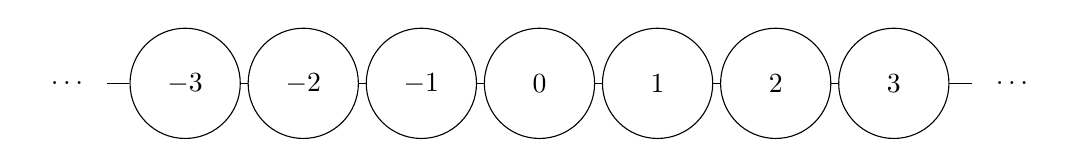
\begin{tikzpicture}[node distance={15mm}, main/.style = {draw, circle}] 
        \node[main,minimum size=1.4cm] (1) {$-3$};
        \node[main,minimum size=1.4cm] (2) [right of=1] {$-2$};
        \node[main,minimum size=1.4cm] (3) [right of=2] {$-1$}; 
        \node[main,minimum size=1.4cm] (4) [right of=3] {$0$};
        \node[main,minimum size=1.4cm] (5) [right of=4] {$1$}; 
        \node[main,minimum size=1.4cm] (6) [right of=5] {$2$};
        \node[main,minimum size=1.4cm] (7) [right of=6] {$3$};

        \node[main,minimum size=1cm, draw=none] (8) [right of=7] {$\ldots$};
        \node[main,minimum size=1cm, draw=none] (9) [left of=1] {$\ldots$};

        \draw (1) -- (2);
        \draw (2) -- (3);
        \draw (3) -- (4);
        \draw (4) -- (5);
        \draw (5) -- (6);
        \draw (6) -- (7);
        
        \draw (1) -- (9);
        \draw (7) -- (8);
        
    \end{tikzpicture}

    v
    

    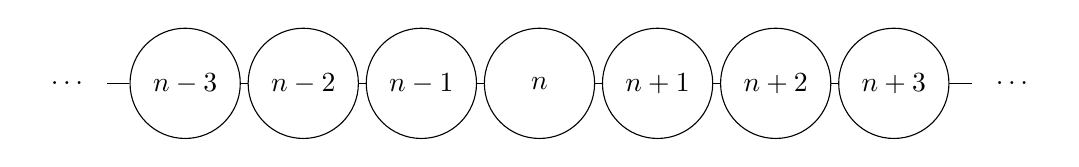
\begin{tikzpicture}[node distance={15mm}, main/.style = {draw, circle}] 
        \node[main,minimum size=1.4cm] (1) {$n-3$};
        \node[main,minimum size=1.4cm] (2) [right of=1] {$n-2$};
        \node[main,minimum size=1.4cm] (3) [right of=2] {$n-1$}; 
        \node[main,minimum size=1.4cm] (4) [right of=3] {$n$};
        \node[main,minimum size=1.4cm] (5) [right of=4] {$n+1$}; 
        \node[main,minimum size=1.4cm] (6) [right of=5] {$n+2$};
        \node[main,minimum size=1.4cm] (7) [right of=6] {$n+3$};

        \node[main,minimum size=1cm, draw=none] (8) [right of=7] {$\ldots$};
        \node[main,minimum size=1cm, draw=none] (9) [left of=1] {$\ldots$};

        \draw (1) -- (2);
        \draw (2) -- (3);
        \draw (3) -- (4);
        \draw (4) -- (5);
        \draw (5) -- (6);
        \draw (6) -- (7);
        
        \draw (1) -- (9);
        \draw (7) -- (8);
        
    \end{tikzpicture}.

    Hitro se prepričamo, da za vsak $n \in \Z$ velja $\rho_n(x) = n + x \neq x$ za poljuben $x \in V$
    in posledično tudi $\{\rho_n(x), \rho_n(y)\} = \{x + n, y + n\} \neq \{x, y\}$ za poljubne $\{x, y\} \in E$,
    torej je to primer prostega delovanja na grafu.
\end{zgled}

Izkaže se, da ta zgled ni nobena partikularnost, za poljubno grupo namreč velja naslednji izrek.

\begin{izrek}
\label{izr:cayleyFreeOrder}
    Naj bo $G$ grupa in $S$ neka množica generatorjev $G$. Potem je delovanje $G$ na \cay{G}{S} z levo translacijo
    $$
    g \cdot v = gv
    $$
    prosto natanko tedaj, ko $S$ ne vsebuje nobenega elementa reda $2$.
\end{izrek}

\begin{proof}
\label{dkz:prostoDelRed}
    Ker velja $g \cdot g' = gg'$ po definiciji delovanja in $gg' = g' \Longleftrightarrow g = e$ zaradi dejstva da sta $g$ in $g'$ elementa grupe $G$,
    je delovanje $G$ na vozliščih \cay{G}{S} vedno prosto, kar zadosti prvemu delu definicije za prosto delovanje na grafu. Dovolj je torej, da dokažemo ekvivalentnost drugega dela definicije.
    
    Pokažimo, da v primeru, da delovanje ni prosto, \cay{G}{S} vsebuje element reda $2$. Naj bo $g \in G$ in naj bo $\{v, v'\}$ povezava v \cay{G}{S} za katerega velja $\{v, v'\} = g \cdot \{v, v'\} = \{g \cdot v, g \cdot v'\}$ (druga enakost je definicija delovanja). Iz enakosti množic ločimo dva primera:
    \begin{enumerate}
    \item Lahko $g \cdot v = v$ in $g \cdot v' = v'$, kar pa je res le v primeru, da je $g = \varepsilon$, ker je delovanje na vozliščih prosto.
    \item Če pa $g \cdot v = v'$ in $g \cdot v' = v$, po definiciji sosednosti v \cay{G}{S} obstaja $s \in (S \cup S^{-1})\setminus \{\varepsilon\}$, da je $v' = vs$. Sledi:
    $$
	v = g \cdot v' = g \cdot (vs) = g(vs) = (gv)s = (g \cdot v)s = (v')s = (vs)s =vs^{2}    
    $$
    Če zdaj z leve množimo z $v^{-1}$, dobimo željeno enakost $e = s^{2}$. Torej je $s$ iskani element reda $2$.
    \end{enumerate}
    
    Pokažimo še, da iz tega, da v $S$ obstaja element reda $2$, sledi, da delovanje ni prosto. Naj bo $s \in S$ reda $2$. Pri delovanju $G$ na \cay{G}{S} velja 
    $$s \cdot \{e, s\} = \{s \cdot e, s \cdot s\} = \{s, s^{2}\} = \{s, e\}\text{,}$$
    kar pomeni, da obstaja element grupe $G$ ki fiksira neko povezavo, torej po definiciji dano delovanje na grafu ni prosto.
\end{proof}

S teorijo, ki smo jo do sem izpeljali, smo že skoraj pripravljeni podati opis prostih grup z
njihovim delovanjem na drevesih. Od zaključka nas loči le že naslednji izrek.

\begin{definicija}[Vpeto drevo delovanja]
    Naj grupa $G$ deluje na povezanem graf $X$. \textbf{Vpeto drevo delovanja} $G$ na $X$ je podgraf grafa $X$, ki je drevo in vsebuje natanko eno vozlišče vsake orbite delovanja $G$ na vozlišča grafa.
\end{definicija}

\begin{izrek}
\label{izr:vpetoDrevoDel}
    Vsako delovanje grupe na povezanem grafu ima vpeto drevo delovanja.
\end{izrek}

\begin{proof}
    Naj bo $G$ grupa, ki deluje na povezanem grafu $X$. Brez škode za splošnost je $X$ neprazen, saj je drugače prazno drevo iskano vpeto drevo delovanja.
    Naj bo $T_{G}$ družina poddreves $X$, ki vsebujejo največ en element vsake orbite delovanja $G$.
    Družina $T_{G}$ je delno urejena za relacijo podgrafa, neprazna (vsebuje prazno drevo), vsaka veriga v $T_{G}$ pa ima zgornjo mejo (konkretno unijo vseh elementov verige).
    Po Zornovi lemi sledi, da $T_{G}$ vsebuje maksimalni element $T$. Ker je $X$ neprazen je tudi $T$ neprazen.

    Zdaj pokažimo, da je $T$ vpeto drevo delovanja. Denimo, da $T$ ni vpeto drevo delovanja.
    Potemtakem obstaja neko vozlišče $v$, da nobeno od vozlišč v orbiti $G \cdot v$ ni vozlišče v $T$. S pomočjo vozlišča $v$ bomo poiskali vozlišče $v_{0}$, za
    katerega bo veljalo, da nobeno od vozlišč v orbiti $G \cdot v_{0}$ ni v $T$, dodatno pa ima $v_{0}$ sosedno vozlišče, ki je v grafu $T$, iz česar bo sledilo protislovje.

    Ker je $X$ povezan obstaja pot $p$, ki povezuje neko vozlišče $u \in T$ z $v$. Naj bo $v'$ prvo vozlišče v poti $p$, da $v' \notin T$. Ločimo dva primera:
    \begin{enumerate}
        \item Nobeno izmed vozlišč v $G \cdot v'$ ni v $T$. Potem je to iskano vozlišče $v_{0} := v'$.
        \item Obstaja $g \in G$, da $g \cdot v' \in T$. Označimo s $p'$ pot med $v'$ in $v$, ter z $g \cdot p'$ pot med $g \cdot v'$ in $g \cdot v$, kjer smo
              vsako vozlišče poti $p'$ ``premaknili`` z delovanjem $g$. Ker je tako premaknjen $g \cdot v' \in T$, pot $g \cdot p'$ pa krajša od poti $p$, lahko
              postopek induktivno nadaljujemo, dokler ne najdemo želenega vozlišča (vozlišče zagotovo najdemo, ker za $v$ noben element $G \cdot g \cdot v = G \cdot v$ ni v $T$).
    \end{enumerate}

    Naj bo zdaj $v$ vozlišče, za katerega noben element $G \cdot v$ ni v $T$ in ima soseda $u \in T$. Če zdaj drevesu $T$ dodamo vozlišče $v$ in povezavo $\{u, v\}$
    dobimo drevo v $T_{G}$, ki vsebuje $T$ kot pravo poddrevo, kar je skregano s trditvijo zornove leme, da je $T$ maksimalno. Torej je $T$ vpeto drevo delovanja grupe $G$ na povezanem grafu $X$.
\end{proof}

\section{Delovanje prostih grup na drevesih}

Pokažimo zdaj, da lahko proste grupe ekvivalentno opišemo z delovanjem na drevesih.
Spodnji izrek nam poda geometrijski opis prostih grup,
kot posledico, pa poda tudi zelo eleganten dokaz trditve, da so podgrupe proste grupe tudi same proste grupe,
ki pa je žal izven obsega tega članka.

Če bralca zanima dokaz omenjene trditve in nadaljevanje teorije prostih grup naj se obrne na sekcijo 4.2.3 v članku \cite{Loh}.

\begin{izrek}
    Grupa je prosta natanko tedaj, ko ima neko prosto delovanje na nepraznem drevesu.
\end{izrek}

\begin{proof}
    $(\Longrightarrow)$

    Naj bo $F$ prosta grupa, prosto generirana z množico $S \subset F$. Po izreku \ref{izr:freeCayleyTree} je njen Cayleyev graf \cay{F}{S} (neprazno) drevo. Po izreku \ref{izr:cayleyFreeOrder} je delovanje $F$ na \cay{F}{S} z levo translacijo prosto natanko tedaj, ko v $S$ ni elementa reda $2$. Uporabimo univerzalno lastnost prostih grup, da se prepričamo da $S$ res nima elementov reda $2$.
    
    Naj bo $\varphi : S \longrightarrow \Z$ poljubna preslikava, za katero velja, da noben $s \in S$ ne slika v $0$. Po univerzalni lastnosti jo lahko dopolnemo do homomorfizma $\overline{\varphi} : F \longrightarrow \Z$. Če $s \in S$ reda $2$, mora red elementa $\overline{\varphi}(s)$ deliti $2$. Red elementa $\overline{\varphi}(s)$ 	ne more biti $2$, saj $(\Z, +)$ ne vsebuje elementov reda 2. Hkrati pa red elementa $\overline\varphi(s)$ ne more biti $1$, ker je v $\Z$ edini element reda $1$ element $0$, ki pa po izbiri $\varphi$ ni slika nobenega $s \in S$ (Spomnimo se, da $\overline\varphi|_{S}$ sovpada s $\varphi$).
    Na isti način bi lahko pokazali, da v prosti grupi noben element ne more imeti končnega reda.
    
    Torej je delovanje proste grupe $F$ na drevesu \cay{F}{S} z levo translacijo prosto.

    $(\Longleftarrow)$
    
    Naj ima grupa $G$ neko prosto delovanje na drevesu $T$. Po izreku \ref{izr:vpetoDrevoDel} za to delovanje obstaja vpeto drevo delovanja.

    Ideja dokaza je, da znotraj grafa $T$ kontraktiramo $T'$ in vsako njegovo translacijo $g \cdot T'$ (kjer $g \in G$) vsako v eno samo vozlišče.
    Na tako dobljeni graf bomo nato lahko gledali kot na graf \cay{G}{\St}, s čimer bomo dobili kandidata za množico $S$. Da $S$ res prosto generira $G$, pa bo sledilo po izreku \ref{izr:cayleyFreeCycle}.

    Preden začnemo s konstrukcijo kandidata poimenujmo z besedno zvezo \textbf{esencialne povezave} povezave v drevesu $T$, ki niso vsebovane v $T'$,
    eno izmed vozlišč med katerima potekajo, pa je vsebovano v $T'$
    (drugo vozlišče zagotovo ne more biti vsebovano v $T'$, saj bi drugače $T$ vseboval cikel).

    Začnimo zdaj s \textit{konstrukcijo kandidata} $S \subset G$. Naj bo $e = \{u, v\}$ esencialna povezava $T$. Brez škode za splošnost je $u \in T'$ in $v \notin T'$.
    Ker je $T'$ vpeto drevo delovanja, obstaja $g_{e} \in G$, da $g_{e}^{-1} \cdot v \in T'$.
    Dodatno, ker orbita $G \cdot v$ vsebuje natanko en element v $T'$ in ker $G$ prosto deluje na $T$, sledi, da je $g_{e}$ enolično določen.

    Definirajmo
    $$
    \St := \{g_e \in G\;|\;e\;\text{je esencialna povezava}\;T \}\text{.}
    $$

    Za množico $\St$ velja:
    \begin{enumerate}
        \item Po konstrukciji enota ni vsebovana v $\St$.
        \item $\St$ ne vsebuje elementov reda $2$.
        
        Če $g_e \in \St$ reda $2$ za esencialno povezavo $e = \{u, v\}$ kot zgoraj, sledi
        $u_0 := g_e^{-1} \cdot v = g_e \cdot v \in T'$. Povezavo $e$ slikamo v $g_e \cdot e = \{g_e \cdot u, u_0\}$
        \begin{enumerate}
            \item Če $u = u_0$, sledi $g_e \cdot e = e$, kar je protislovje s predpostavko o prostem delovanju.
            \item Če $u \neq u_0$, sledi $\{u_0, g_e \cdot u\} \in g_e \cdot T = T$ (delovanje $g_e$ je automorfizem).
            Znotraj $T'$ obstaja pot med $u_0$ in $u$, znotraj $g_e \cdot T'$ (disjunkten s $T'$) pa pot med $g_e \cdot u$ in $v$.
            Ker sta $e$ in $g_e \cdot e$ povezavi $T$ imamo v $T$ cikel, kar je protislovje s tem, da je $T$ drevo.
        \end{enumerate}

        \item Če sta $e$ in $e'$ esencialni povezavi, za kateri sta $g_e = g_{e'}$, potem $e = e'$ ($T$ je drevo, zato, kot zgoraj, ne moreta obstajati dve različni povezavi med povezanima $T'$ in $g_e \cdot T' = g_{e'} \cdot T'$).
        \item Če je $g \in \St$, denimo $g = g_e$ za neko esencialno povezavo $e$, potem je tudi $g^{-1} \cdot e$ esencialna povezava in $g^{-1} = g_{g^{-1} \cdot e} \in \St$.
        
        Z drugimi besedami, obstaja podmnožica $S \subset \St$, da velja:
        \begin{align*}
            S \cap S^{-1} = \emptyset && \text{in} && |S| = \frac{|\St|}{2} = \frac{1}{2} \cdot \#\;\text{esencialnih povezav}\;T\text{.}
        \end{align*}
    \end{enumerate}

    V naslednjem koraku pokažimo, da $\St$ (in posledično $S$) \textit{generira} $G$.
    Naj bo $g \in G$ poljuben in $v \in T'$ poljubno vozlišče. Ker je $T$ povezan, v njem med vozliščema $v$ in $g \cdot v$ obstaja pot $p$.
    Pot $p$ gre skozi več kopij $T'$. Označimo s $g_0 \cdot T', \ldots , g_n \cdot T'$ zaporedne kopije $T'$, skozi katere
    vodi $p$, tako da velja $g_0 = e$, $g_n = g$ in $g_i \neq g_{i+1}$ za vsak $i \in \{0, \ldots, n-1\}$.
    Naj bo zdaj $j \in \{0, \ldots, n-1\}$ poljuben. Ker je $T'$ vpeto drevo delovanja in je $g_i \neq g_{i+1}$, sta kopiji
    $g_j \cdot T'$ in $g_{j+1} \cdot T'$ povezani z neko povezavo $e_j$. Po definiciji je $g_j^{-1} \cdot e_j$ esencialna povezava, kateri smo v $\St$ priredili element
    $$s_j := g_j^{-1}g_{j+1}$$
    (bralec naj se sam prepriča da velja $s_j^{-1} \cdot v \in T'$, kjer $v \in g_j^{-1} \cdot e_j$, $v \notin T'$).

    Vidimo, da velja
    \begin{align*}
        g &= g_n = g_0^{-1} g_n \\
          &= g_0^{-1} g_1 g_1^{-1} g_2 \dotsm g_{n-1}^{-1} g_n \\
          &= s_0 s_1 \dotsm s_{n-1}
    \end{align*}
    in $g$ je element podgrupe generirane s $\St$. Ker je bil $g$ poljuben sledi, da $\St$ generira $G$.
    Tako vidimo, da lahko, ko znotraj $T$ kontraktiramo vse kopije $T'$ vsako v eno samo vozlišče, novo dobljeni graf gledamo kot \cay{G}{\St}
    (kopija $g \cdot T'$ po kontrakciji ustreza elementu $g$).

    Ostane nam le še premislek, da $S \subset \St$, ki smo ga definirali zgoraj \textit{prosto generira} $G$. Po izreku \ref{izr:cayleyFreeCycle} zadošča dokazati, da \cay{G}{S} ne vsebuje ciklov (predpostavki $\forall s,t \in S : s \cdot t \neq e$ smo zadostili s $4$. lastnostjo $\St$),
    kar pa bo držalo, ker lahko v primeru da imamo cikel, \cay{G}{S} razširimo nazaj v $T$, ter pridemo v protislovje s predpostavko, da je $T$ drevo.
    
    Naredimo torej to. Denimo, da obstaja $n \in \N$, $n \ge 3$ za katerega v \cay{G}{S} $=$ \cay{G}{\St} obstaja cikel $g_0, \ldots, g_{n-1}$. Kot zgoraj so
    \begin{align*}
        s_{j+1} &:= g_j^{-1}g_{j+1} \quad j \in \{0, 1, \ldots, n-2\} \\
        s_n &:= g_{n-1}^{-1}g_0
    \end{align*}
    elementi $\St$. Naj bo $e_i$ esencialna povezava med $T'$ in $s_i \cdot T'$ za $i \in \{1, \ldots, n\}$.
    Oglejmo si povezavi $e_i$ in $e_{i+1}$ za $i \in \{1, \ldots, n-2\}$. Njuni translaciji $g_{i-1} \cdot e_i$ in $g_{i} \cdot e_{i+1}$ povezujeta translaciji $g_{i-1} \cdot T'$ z $g_{i} \cdot T'$ ter $g_{i} \cdot T'$ z $g_{i+1} \cdot T'$.
    Ker je $g_i \cdot T'$ drevo, znotraj njega obstaja pot med tistim vozliščem povezav $g_{i-1} \cdot e_i$ in $g_{i} \cdot e_{i+1}$, ki je v $g_{i} \cdot T'$.
    Vidimo torej, da obstaja pot med $g_0 \cdot T'$ in $g_{n-1} \cdot T'$. Ker pa $g_{n-1} \cdot e_n$ povezuje $g_{n-1} \cdot T'$ in $g_0 \cdot T'$ pomeni, da v $T$ obstaja cikel, s čimer smo prišli v iskano protislovje.

\end{proof}

\newpage

% TODO
\section*{Angleško-slovenski slovar strokovnih izrazov}

\geslo{free group}{prosta grupa}

\geslo{free generating set}{množica ki prosto generira}

\geslo{generating set}{množica generatorjev}

\geslo{universal property}{univerzalna lastnost}

\geslo{reduced word}{okrajšana beseda}

\geslo{cayley graph}{cayleyev graf}

\geslo{group action}{delovanje grupe}

\geslo{free action}{prosto delovanje}

\geslo{spanning tree}{vpeto drevo}

\geslo{spanning tree of an action}{vpeto drevo delovanja}

\geslo{essential edge}{esencialna povezava}



\bibliographystyle{plain}
\bibliography{bibliografija}

\end{document}
